
\section{Crowdsourcing}
In order to complete the corpus, we required human sourced elicitations for continuations of the personal narratives presented in the dataset. We decided to exploit crowdsourcing, designing an experimental setup to instruct crowdworkers on how to induce the continuation of the narrative. This is followed by the data collection and an statistical analysis of the crowdsourced eliting questions.
% This section reports a concise overview of the experimental setup for crowdsourcing.
%  This section is comprised of:
% \begin{itemize}
%     \item \textbf{Guidelines design}: Drafting guidelines tailored for the crowdsourcing component of the study and iteratively reviewing them until satisfactory.
%     \item \textbf{User Interface (UI) Design for Crowdsourcing}: Creation of a user-friendly interface incorporating the guidelines previously drafted, ensuring a seamless user experience.
%     \item \textbf{Data collection}: Engaging crowdworkers to participate in the data collection process and collection of responses to our narrative prompts.
%     \item \textbf{Data analysis}: A comprehensive data analysis on the participants' eliciting questions was conducted.
% \end{itemize}
\subsection{Guidelines design}
The formulation of effective guidelines was a fundamental requirement. This step necessitated an iterative process involving the creation of drafts, subsequent reviews, and pilot tests of guidelines. Pilot test were used to gauge the effectiveness of the guidelines in directing workers to generating correct eliciting questions for the continuation of personal narratives. This iterative cycle was repeated until the guidelines reached a level of satisfaction.

\begin{table}[!htbp]
\centering
\caption{Three examples of narratives with highlighted text that represents valence values, which are reported on the right. The sections highlighted in red represent negative values, while in the ones highlighted in green represent positive values. Neutral values corresponding to 0 are not highlighted and not reported.}
\label{tab:dataset-coadapt-highlight-examples}
    \centering
    \begin{tabularx}{\linewidth}{ X | c }
    % \begin{tabular}{p{1.5cm}|p{3cm}|p{5cm}|p{2.5cm}|p{2cm}}
        \toprule
        \multicolumn{2}{c}{\thead{Example of how highlighted text is used to convey valence information}} \\
        \midrule
       \thead{Narrative} & \thead{Valence values} \\
        \midrule
        Ciao, \highLight[highlightgreen]{tutto bene} molto lavoro il questi ultimi giorni. & +1\\[1em]
        % \midrule
        Ritornata dal lavoro \highLight[highlightred]{mia figlia mi dice di aver chiamato il medico perché ha dei dolori alla testa non ha il senso dell'olfatto e del gusto per cui ci siamo un po' allarmati.} & -1 \\[2em]
        % \midrule
        Oggi mi sono dedicata al giardino e all'orto. Sono stanchissima fisicamente ma rilassata mentalmente. Fuori in giardino ho fatto tutte le cose che prima faceva mio marito. Ho sentito quasi fisicamente la sua presenza \highLight[highlightgreen]{e la cosa mi ha rilassato} & +1 \\
        \bottomrule

    \end{tabularx}
\end{table}

After finalising the guidelines, the next step involved translating them into a custom web-based user interface (UI) for the data collection process. One key aspect of our guidelines was the inclusion of the valence values from the CoAdapt dataset. 
As previously mentioned, effective elicitation requires empathy, particularly for sorrowful events. In order to facilitate the crowdworkers in pivoting their questions to emotionally charged events, the valence values were highlighted in the text, with the recommendation to focus on those parts of the narrative. In order to represent effectively to the crowdworkers the positive and negative emotions expressed by the valence, it was decided to highlight negative valences in red and positive valences in green. An illustrative example can be seen in Table \ref{tab:dataset-coadapt-highlight-examples}. These colours were chosen as it is universally accepted that green stands for positive and red for negative. Furthermore, to limit the crowdworkers' cognitive workload, the ECs have not been added.
\begin{table}[!htbp]
\centering
\caption{Table reporting the desired and undesired properties of the elicitations }
\label{tab:dataset-crowdsourcing-guidelines-properties}
    \centering
    % \begin{tabularx}{p{2cm}|p{3cm}|p{5cm}|p{5cm}}
    \begin{tabularx}{\linewidth}{ X | X }
        \toprule
        \thead{Desired properties} & \thead{Undesired properties} \\
        \midrule
         Suggested, but not enforced, focused on the highlighted portions of the narratives, i.e. parts of the narratives with valence. &   Questions on personal opinions. \\[2em]
         Containing feedback signals, such as \emph{"Capisco"} or \emph{"Oh, che bello"} and other signs of active listening. &  Suggestions \\[2em]
         Centered around the narrator, i.e. should not move away from the narrator the focus of the story. &   Hypothetical questions or scenarios. \\[2em]
         Containing explicit references to events that happened in the narrative. &  Questions that move the focus of the conversation away from the narrator.\\[2em]
         Showing empathy to the narrator, for instance with words as \emph{``Mi dispiace"} when sad events are mentioned. \\[2em]
         Short and on point. \\[1em]
         Correct, both grammatically and syntactically. \\[1em]
         Focused on events of the narrative. \\[1em]
        \bottomrule
    \end{tabularx}
\end{table}
% The main purpose of these guidelines was to help workers in producing a good elicitation. Our goals were for the elicitation to be questions with the following properties:
% \begin{itemize}
    
%  Focused on events of the narrative.
%  Suggested, but not enforced, focused on the highlighted portions of the narratives, i.e. parts of the narratives with valence.
%  Containing feedback signals, such as \emph{"Capisco"} or \emph{"Oh, che bello"} and other signs of active listening.
%  Centered around the narrator, i.e. should not move away from the narrator the focus of the story.
%  Containing explicit references to events that happened in the narrative.
%  Showing empathy to the narrator, for instance with words as \emph{"Mi dispiace"} when sad events are mentioned.
%  Short and on point.
%  Correct, both grammatically and syntactically.
% % \end{itemize}
% % On the other hand, we explicitly required our elicitation not to be any of the following:
% % \begin{itemize}
%  Questions on personal opinions.
%  Suggestions.
%  Hypothetical questions or scenarios.
%  Questions that move the focus of the conversation away from the narrator.
% % \end{itemize}
This task places a large emphasis on the examples included in the guidelines because, during a pilot test, it was found that many crowdworkers try to complete the task as quickly as possible, giving only a light read to the guidelines and skipping directly to the examples. 
\begin{table}[ht]
\centering
\caption{Table reporting an example that was provided to the users with correct and incorrect elicitation.}
\label{tab:dataset-crowdsourcing-guidelines}
    \centering
    % \begin{tabularx}{p{2cm}|p{3cm}|p{5cm}|p{5cm}}
    \begin{tabularx}{\linewidth}{ p{1.5cm} | X | p{2.5cm} | p{3cm} }
        \toprule
        \multicolumn{4}{c} { \thead{Examples of elitictations}}\\
        \midrule
        \thead{Narrative} & \multicolumn{3}{p{14.5cm}}{ \hlgreen{Oggi è stata una bella giornata. Mia moglie mi ha detto che sta aspettando un bambino!} Sono super felice! Mi chiedo se sarò un bravo padre. \hlred{Mio padre non è stato molto presente quando ero un bambino.}}\\
        \midrule
        \thead{Example} & \thead{Text} & \thead{Evaluation} & \thead{Explaination} \\
        % \arrayrulecolor{lightgray}
        \midrule
        \thead{1} & Sono felice di sentirlo. Sapete già se si tratta di un maschio o di una femmina ? &	\textbf{CORRETTO} &	Segue tutte le linee guida \\[2em]
        % \midrule
        \thead{2} &	Oh capisco. Cosa mi racconti? &	\textbf{ERRATO} &	Non esplora la narrativa, troppo generica \\
        % \arrayrulecolor{black}
        \bottomrule
    \end{tabularx}
\end{table}

Table \ref{tab:dataset-crowdsourcing-guidelines} reports examples of good and bad elicitating questions for a given narrative that were given to the crowdworkers. 
%Initially, the examples provided were found to be ineffective, as they did not highlight the common issues faced by the crowdworkers. Therefore, after some internal testing, better examples that guide the crowdworkers through typical caveats of the task were devised.

% The main purpose of these guidelines was to help workers in producing a good elicitation. Our goals were for the elicitation to be questions with the following properties:
% \begin{itemize}
%     \item Focused on events of the narrative.
%     \item Suggested, but not enforced, focused on the highlighted portions of the narratives, i.e. parts of the narratives with valence.
%     \item Containing feedback signals, such as \emph{``Capisco"} or \emph{``Oh, che bello"} and other signs of active listening.
%     \item Centered around the narrator, i.e. should not move away from the narrator, the focus of the story.
%     \item Containing explicit references to events that happened in the narrative.
%     \item Showing empathy to the narrator, for instance, with words as \emph{``Mi dispiace"} when sad events are mentioned.
%     \item Short and on point.
%     \item Correct, both grammatically and syntactically.
% \end{itemize}
% On the other hand, we explicitly required our elicitation not to be any of the following:
% \begin{itemize}
%     \item Questions on personal opinions.
%     \item Suggestions.
%     \item Hypothetical questions or scenarios.
%     \item Questions that move the focus of the conversation away from the narrator.
% \end{itemize}
A brief recap of the desired properties of the eliciting questions is reported in Table \ref{tab:dataset-crowdsourcing-guidelines-properties}.
The table reports a few scenarios, such as requests for personal opinions or hypothetical conditions, which should be avoided because, in the internal testing, it was found that those types of questions may induce the narrator to start a new narrative with a different set of events. This is not desirable as the goal of those eliciting questions is to explore the current narrative and not to start a new one.
% Those examples were part of the guidelines that were given to the crowdworkers.
\subsection{User Interface (UI) Design for Crowdsourcing}
\begin{figure}[!htbp]
    \centering
    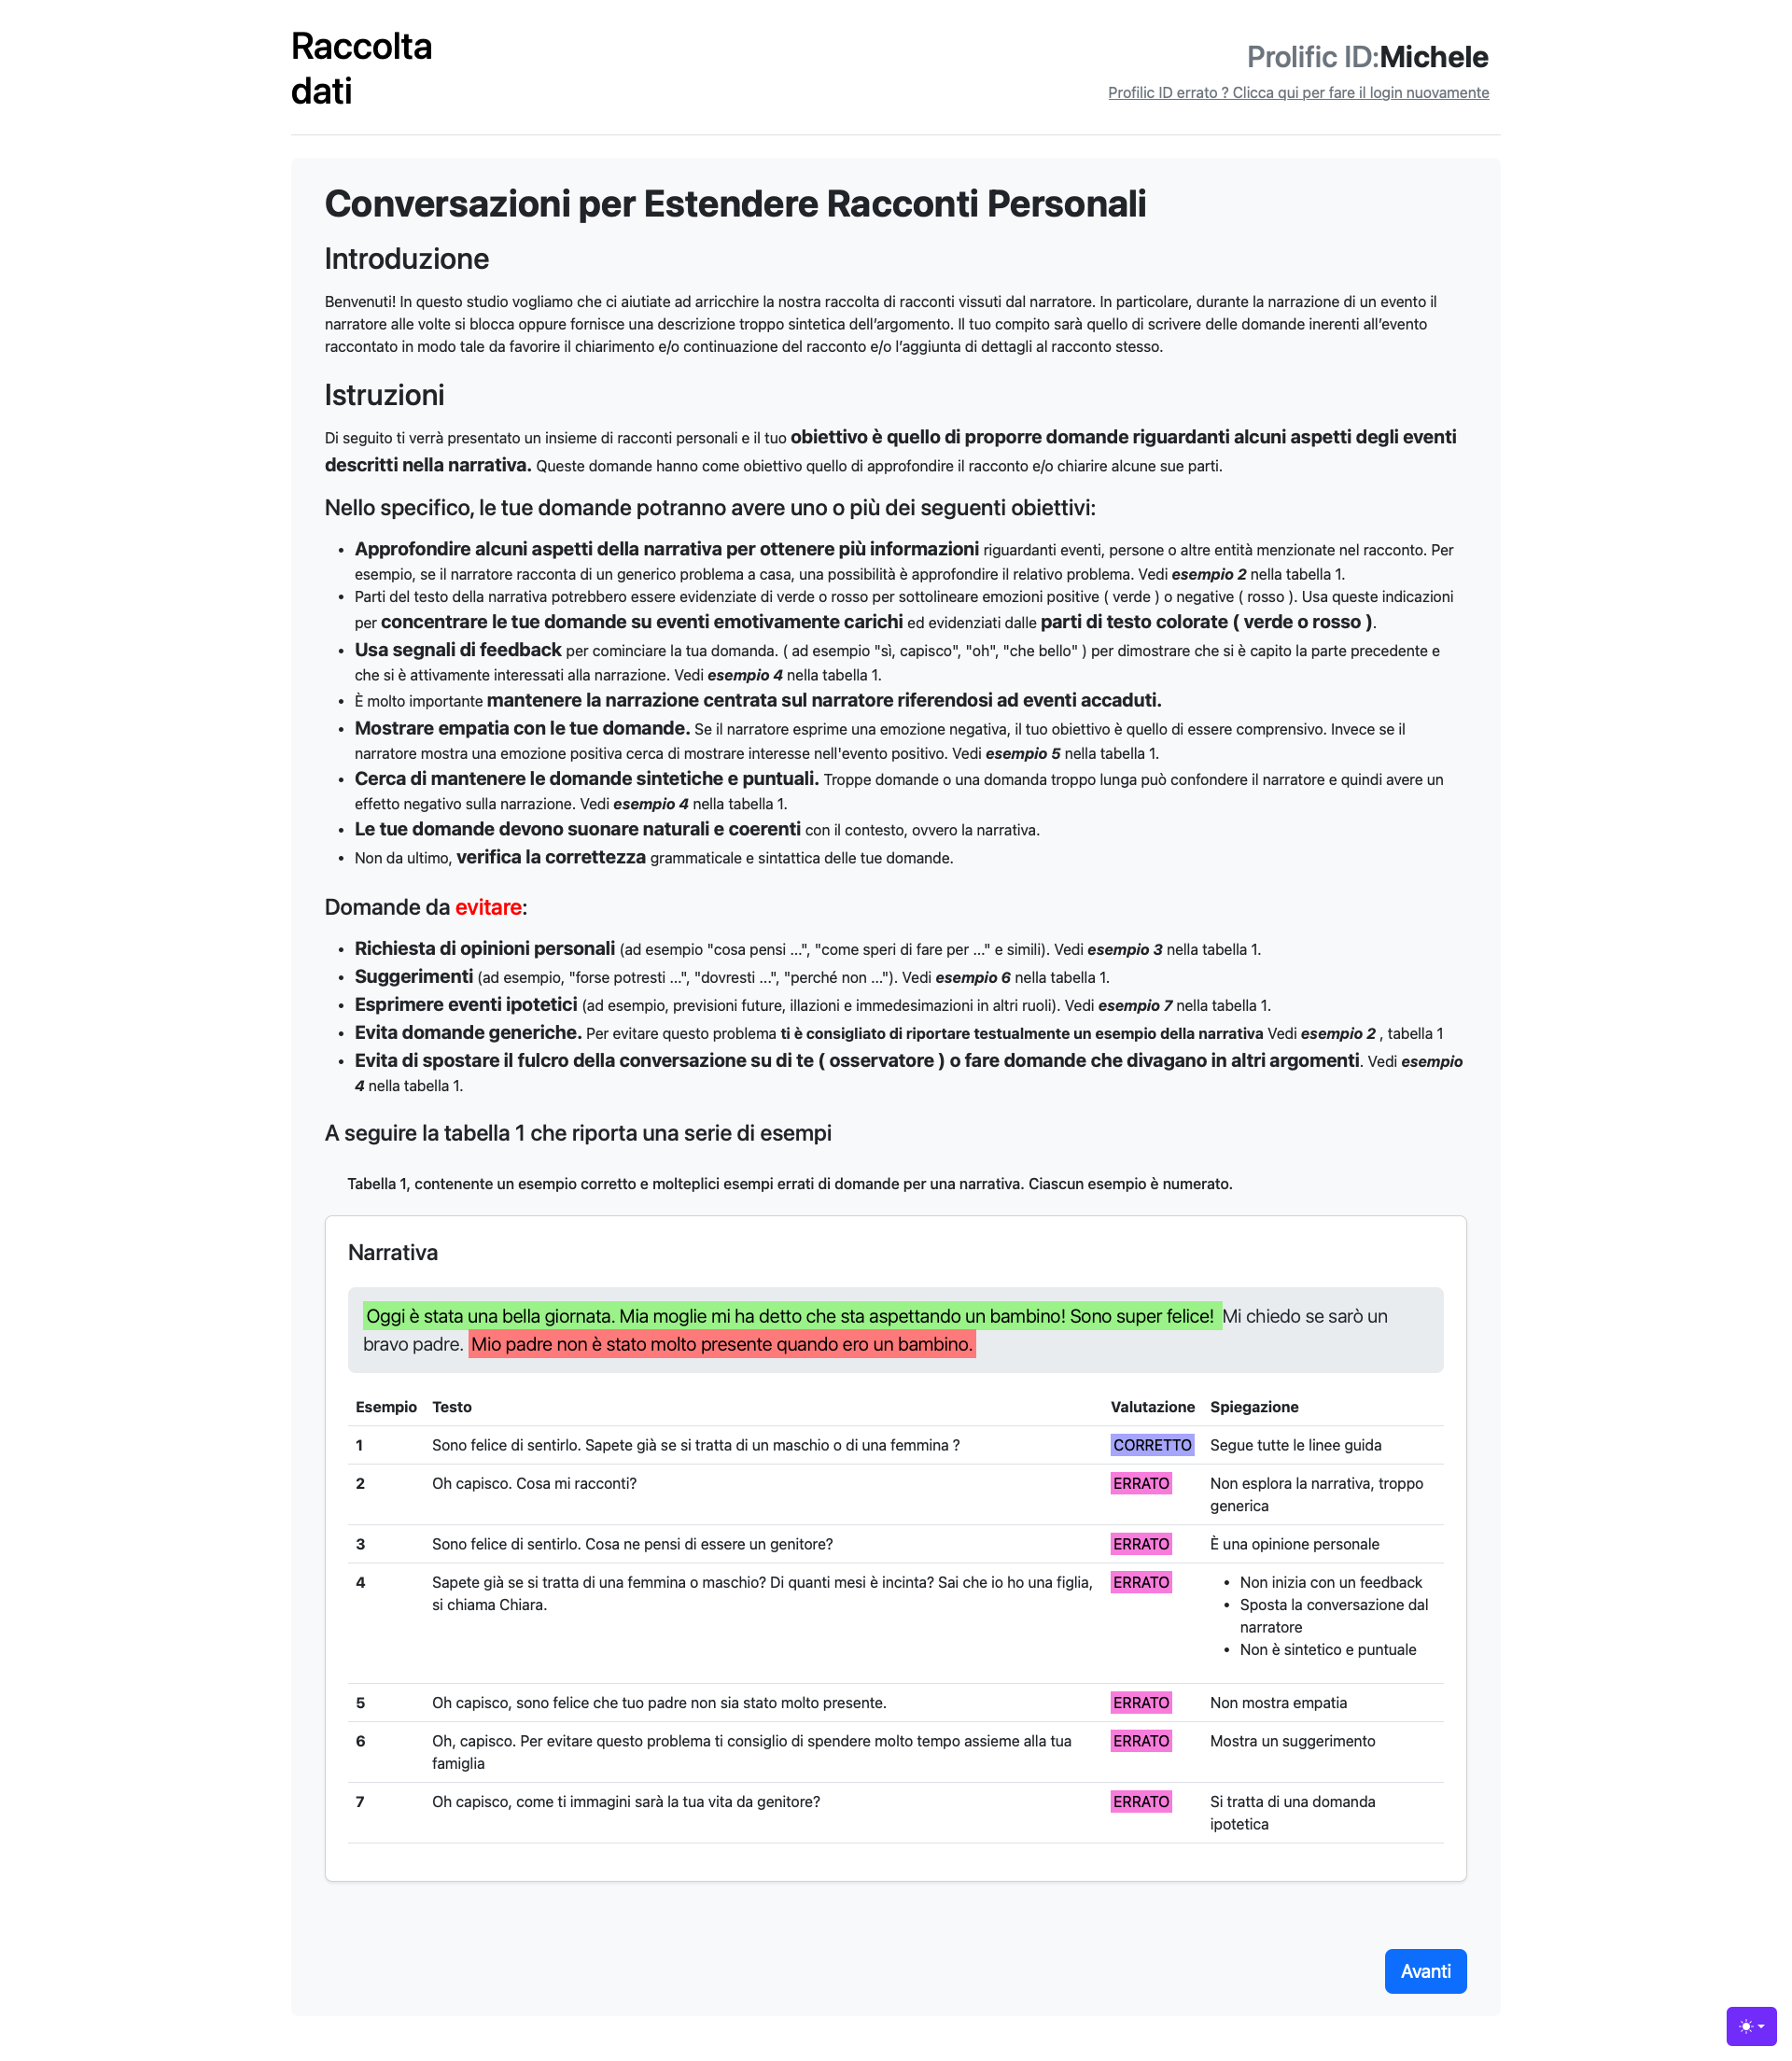
\includegraphics[width=1\linewidth]{assets//imgs/UI-guidelines.png}
    \caption{Image of the Web UI that was shown to the crowdworkers for the guidelines. This page was shown initially to the user and was available for later review with the press of a button.}
    \label{fig:data_collection_web:1}
\end{figure}

\begin{figure}[!htbp]
    \centering
    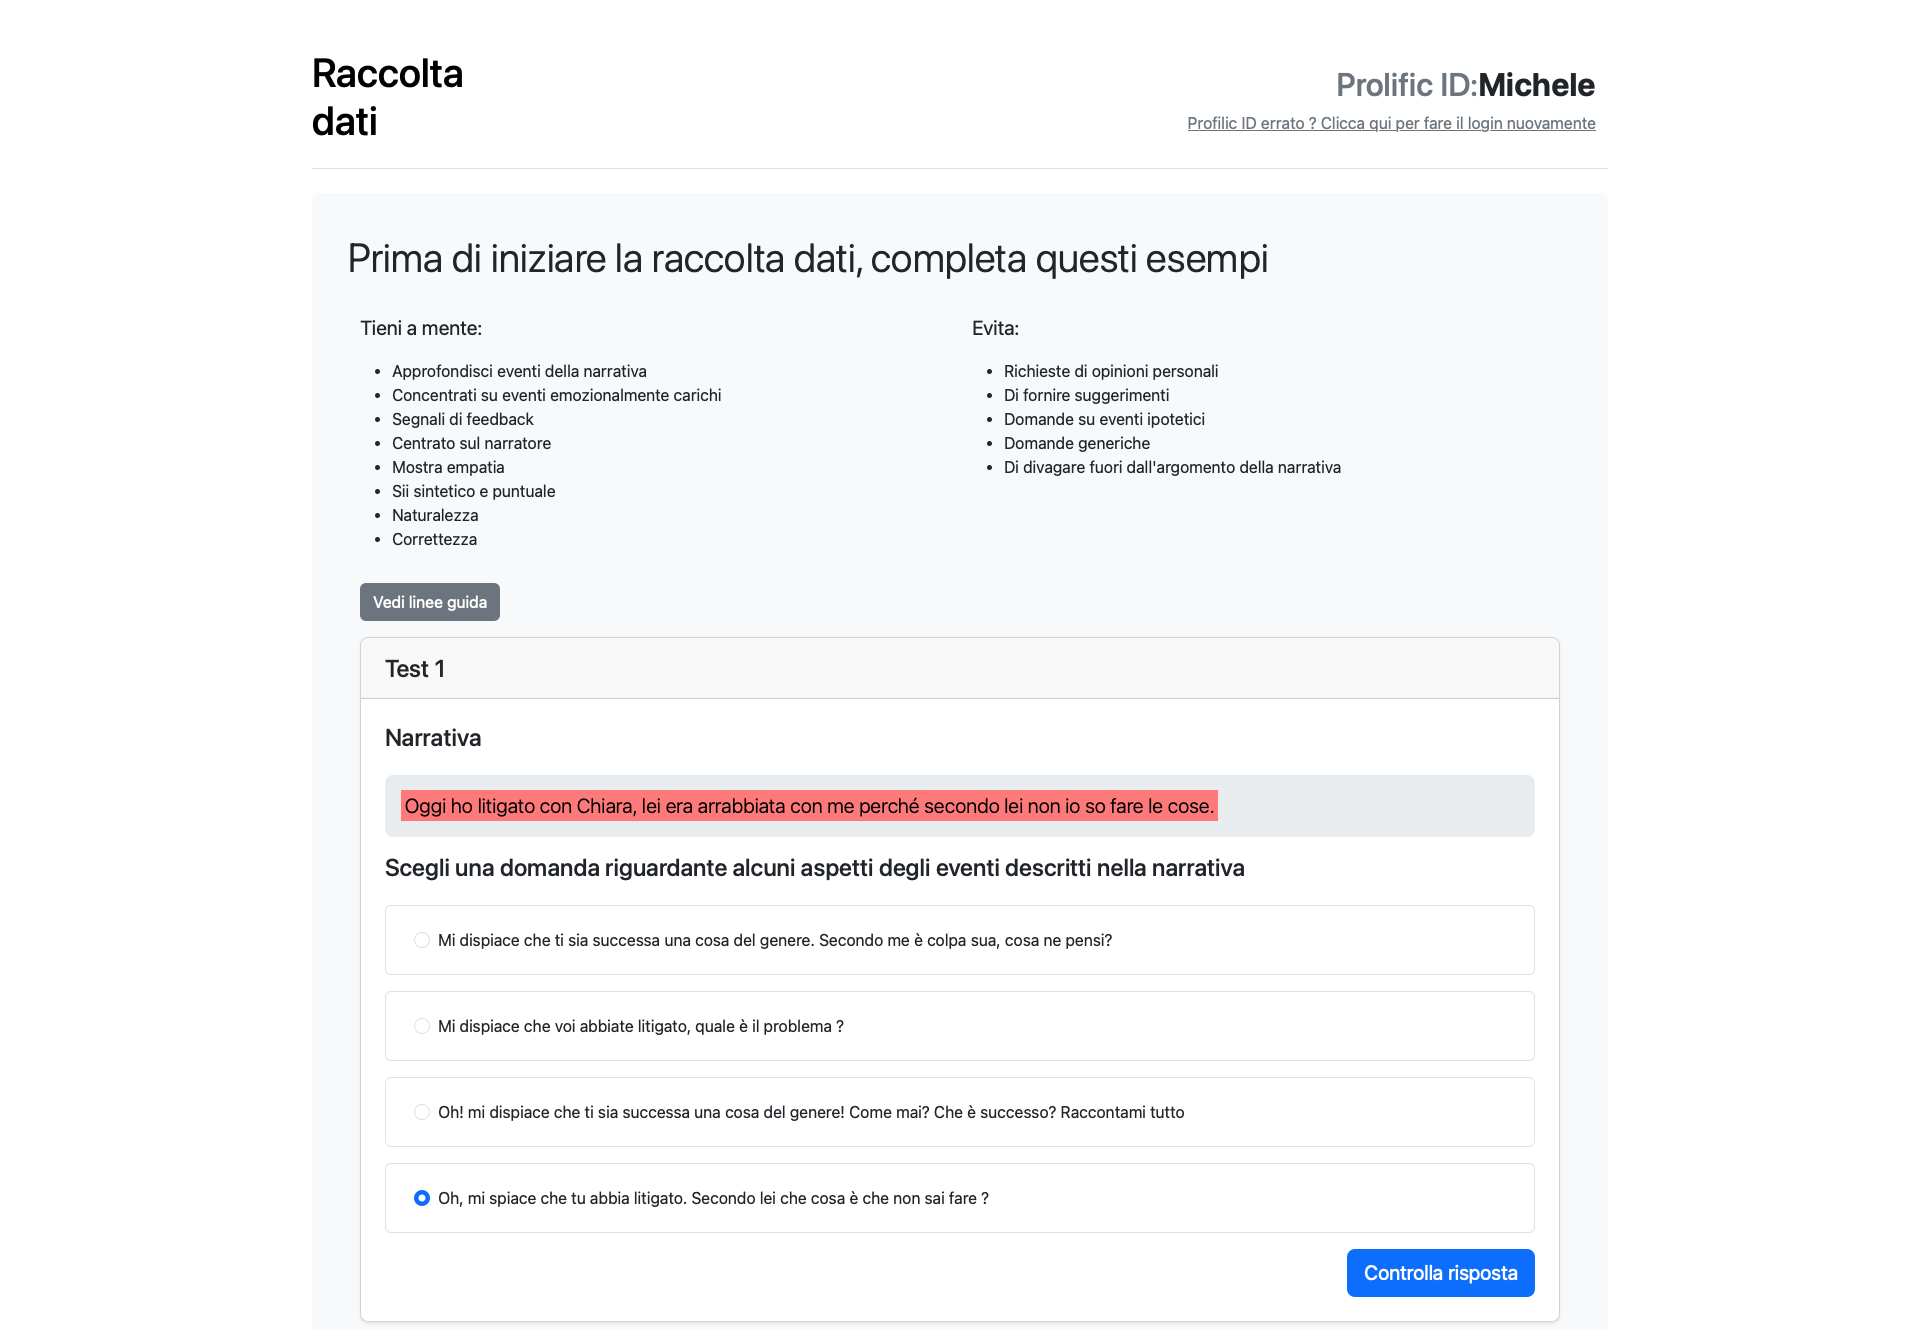
\includegraphics[width=1\linewidth]{assets//imgs/UI-examples-1.png}
    \caption{Image of the Web UI that was shown to the crowdworkers as training examples. After the guidelines, 4 examples similar to this one were assigned to the crowdworkers in order to train them.}
    \label{fig:data_collection_web:2}
\end{figure}
\begin{figure}[!htbp]
    \centering
    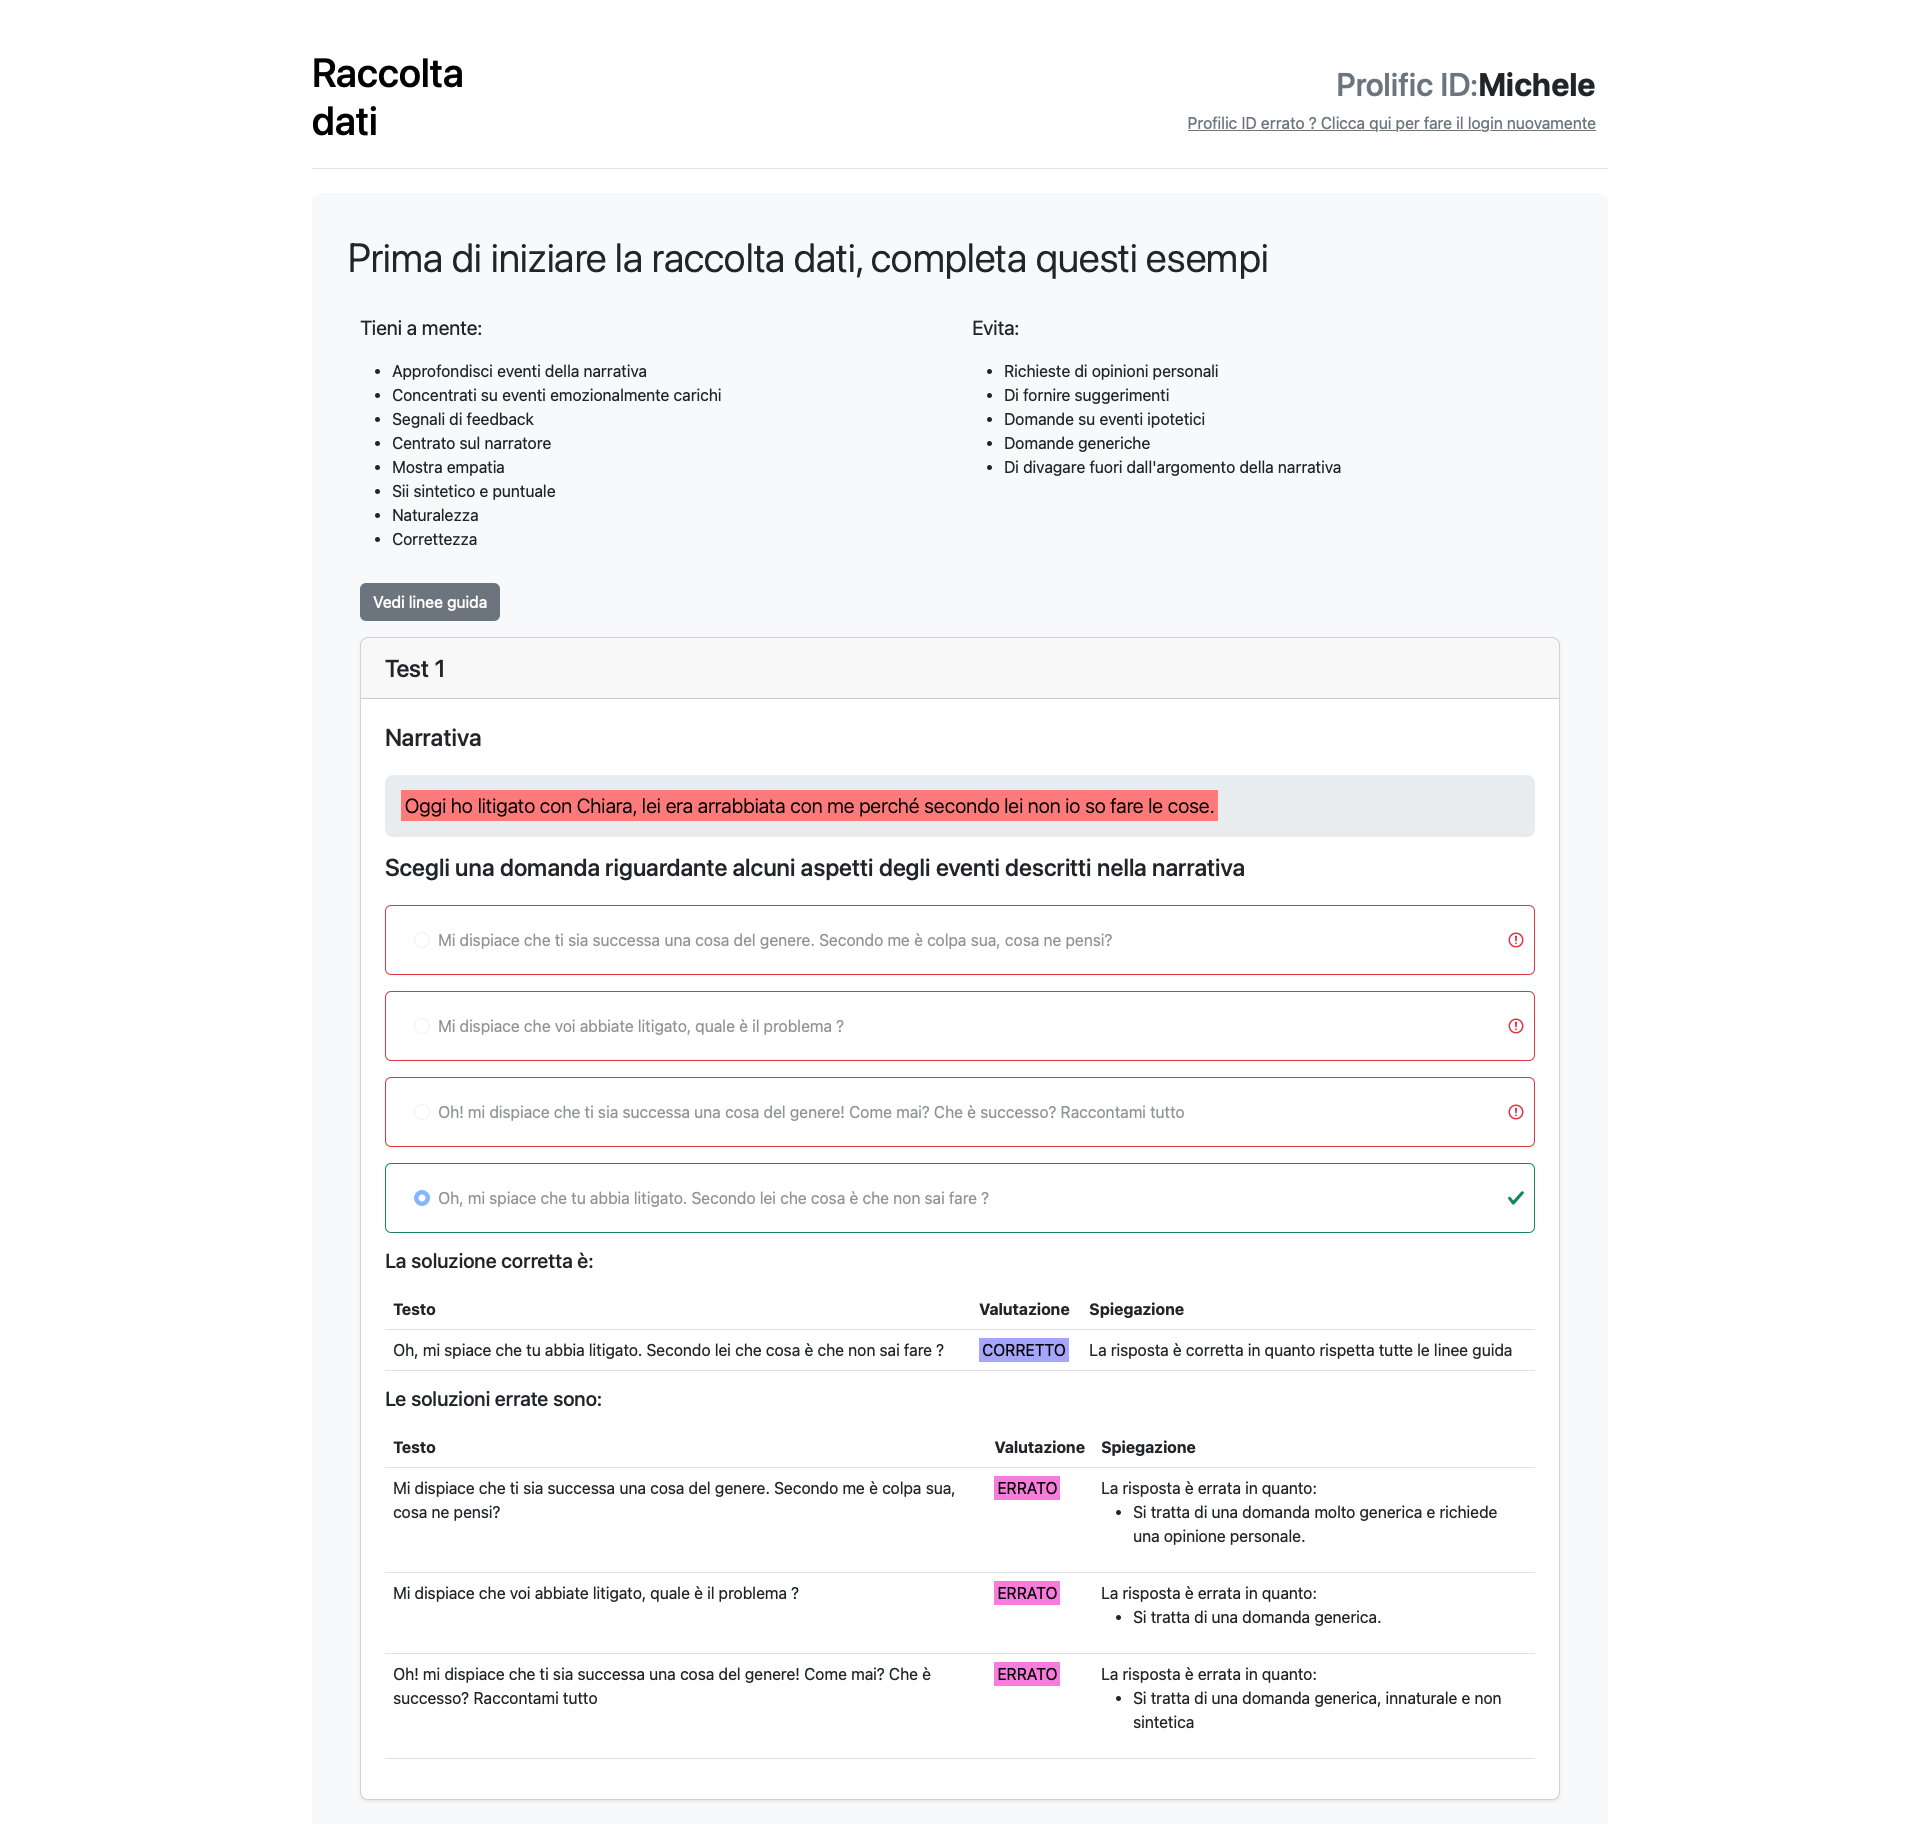
\includegraphics[width=1\linewidth]{assets//imgs/UI-examples-completed-1.png}
    \caption{Image of the Web UI that was shown to the crowdworkers as training examples. After each user inputs an answer, an example of a correct answer this the motivation was shown to train the crowdworkers against typical mistakes.}
    \label{fig:data_collection_web:3}
\end{figure}
\begin{figure}[!htbp]
    \centering
    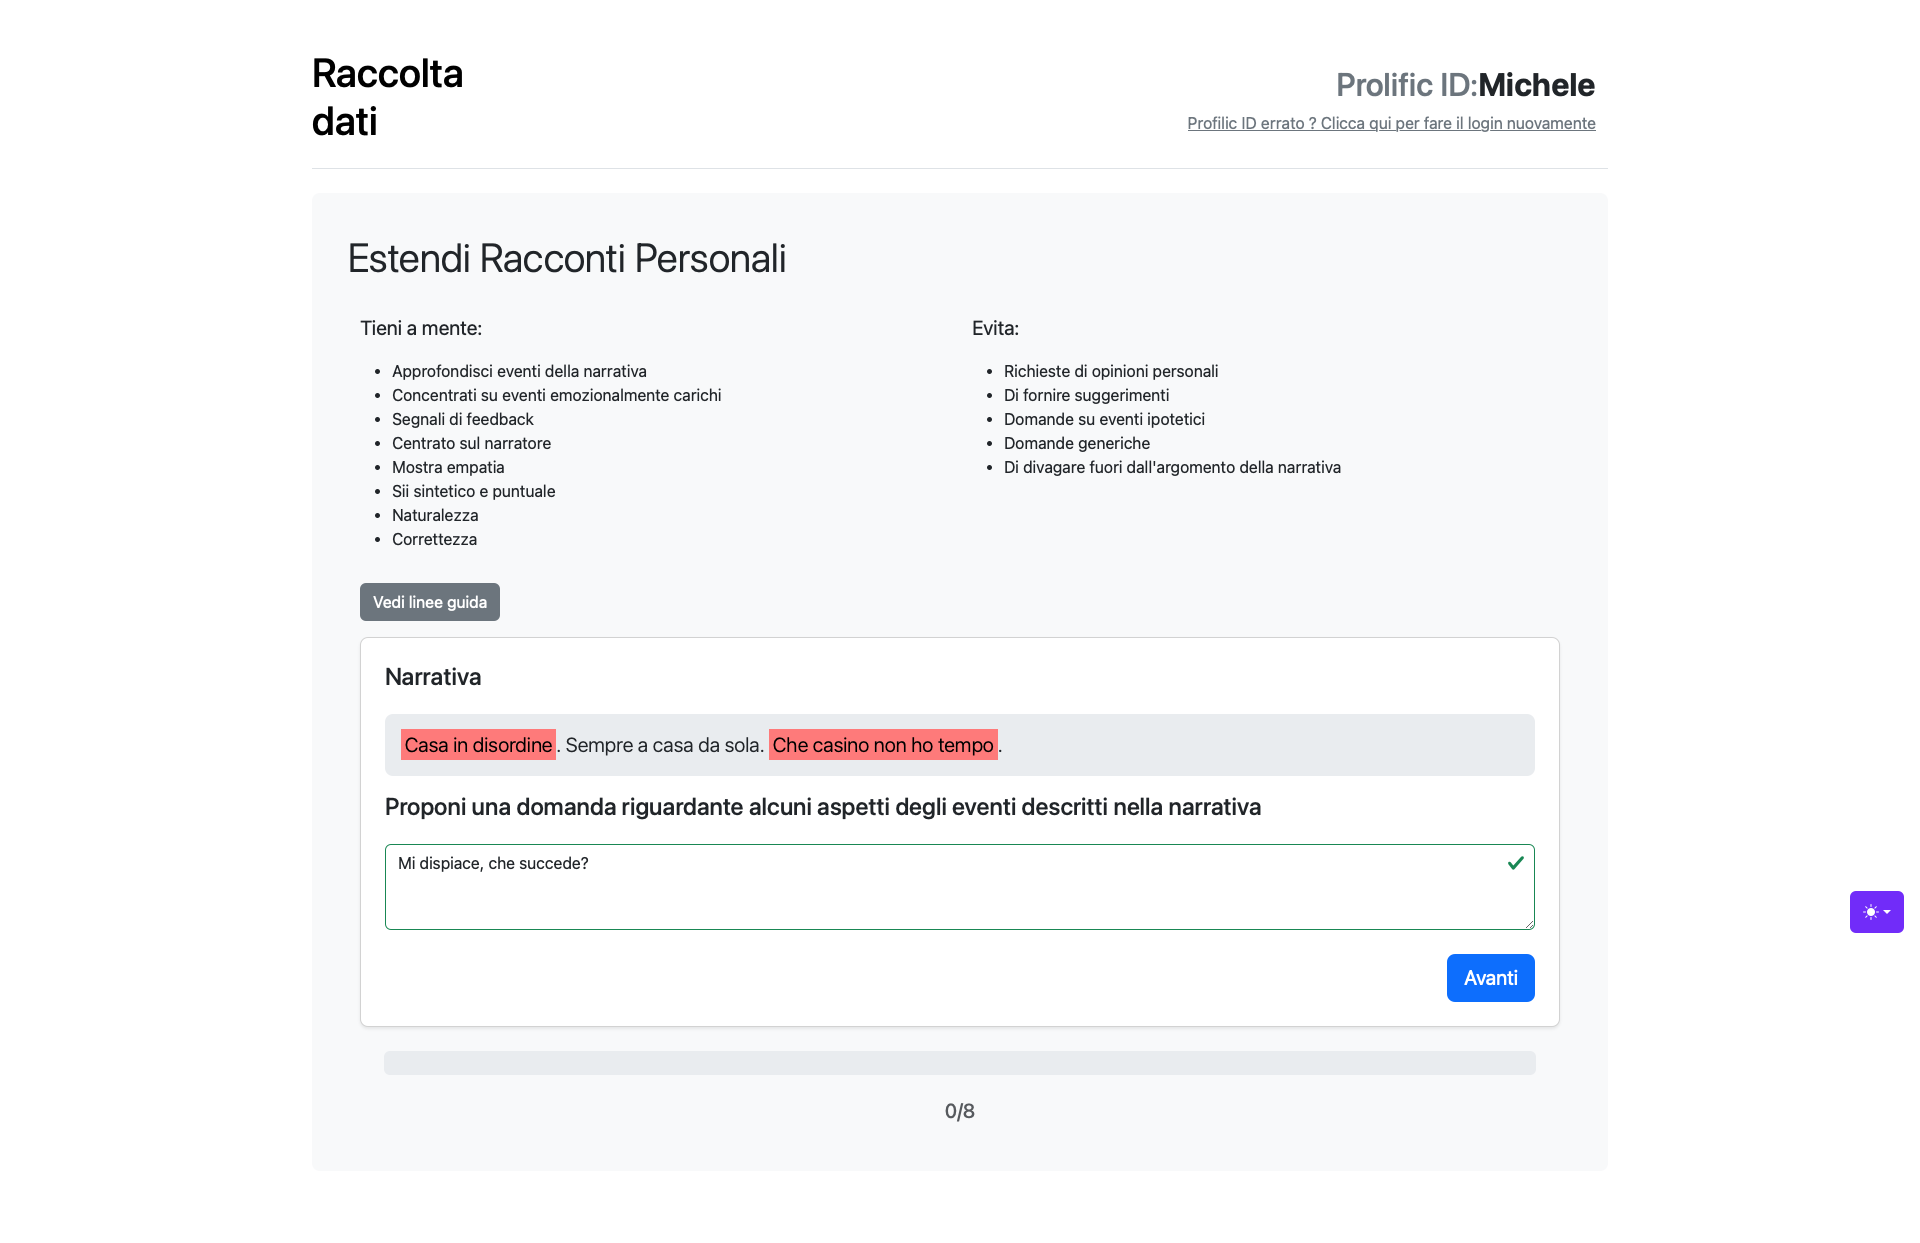
\includegraphics[width=1\linewidth]{assets//imgs/UI-datacollection.png}
    \caption{Image of the Web UI that was shown to the crowdworkers for the actual data collection process.}
    \label{fig:data_collection_web:4}
\end{figure}

For the UI, the selection of the design framework was founded upon Bootstrap \cite{bootstrap}. Bootstrap was chosen due to its user-friendly nature, ease of development, and contemporary design elements. Testing was conducted on multiple platforms, encompassing mobile devices, various web browsers, and distinct operating systems to ensure optimal user experience across diverse devices.
A few pages of the UI are reported. In Figure \ref{fig:data_collection_web:1} is shown the UI used to convey the guidelines, in Figure \ref{fig:data_collection_web:2} and \ref{fig:data_collection_web:3} are shown the examples that were used as training examples for the users. Finally, in Figure \ref{fig:data_collection_web:4} is reported the UI used for the actual data collection.

The colours used in the palette are material \cite{material}, with modern rounded corners and no sharp edges, keeping the design as minimal as possible. Colours for the highlighted text are a pale shade of red and green, \# F77A7B (\redbg{\hspace{1em}}) and \# 9AF288 (\greenbg{\hspace{1em}}). These colours were chosen due to their light tint and their high contrast on black text, allowing the text underneath the highlighted selection to be easily read.


\subsection{Data Collection}
\label{cha:methodology-data-collection}
Subsequently, upon the successful completion of the user interface, the data collection phase was initiated. Prolific, a reputable platform \cite{prolific} for data collection, was employed for this purpose. From this platform, only native Italian speakers were selected as eligible to undertake the task, due to the fact that our corpus is written in the Italian language.

The data collection process started with an initial pilot test, verifying accuracy and identifying any potential procedural errors. Once those were fixed, the data collection was started. The data collection was conducted in multiple batches, remunerating participants at a rate of £12 per hour. To prevent participant fatigue, each batch included a range from 5 to 8 narratives, with an estimated completion time of approximately 20 minutes per batch. In order to give roughly the same amount of load to each worker, a stratified sampling approach was used on the narrative lengths, giving each worker a similar amount of words to read. At the same time, to ensure consistency and elicit agreement among narrators, the first narrative for each batch across a set of batches was intentionally kept identical for different annotators. This first narrative was also shorter in length compared to subsequent narratives. This approach was employed for the dual purpose of manually verifying consensus among narrators regarding their elicitation topics on the same narrative and also serve as a warm-up exercise for the crowdworkers. This meant that there were a few narratives with multiple eliciting questions.

Following each run, each eliciting question was individually inspected and proofread in order to reject any unreliable data, resulting in the exclusion of only one set of answers.

% In total, a sum of $\sim$ £400 was disbursed as compensation for participant contributions.

\subsection{Data Analysis}
\label{cha:methodology-crowdsourcing-data-analysis}

\begin{table}[ht]
\centering
\caption{Table reporting the statistics computed from the answers collected from the dataset.}
\label{tab:dataset-data-collection-statistics}
    \centering
    \begin{tabular}{l|rrr}
    % \begin{tabularx}{\linewidth}{  X | X | X | X }
        \toprule
        \thead{Statistics} & \thead{Train Set} & \thead{Test Set} & \thead{Overall Set}\\
        \midrule
        Number of narratives& 419 & 57 & 476 \\
        Number of answers collected & 510 & 84 & 594\\[1em]
        
        Average answer length & 12.07 & 10.42  & 11.81 \\
        Standard deviation on answer length & 6.61 & 5.12 & 6.43 \\[1em]
        Average guidelines reading time& 428.97 s & 291.17 s & 401.41 s \\
        Standard deviation on guidelines reading time& 336.41 s & 126.49 s & 311.09 s \\[1em]
        Average narrative elicitation time & 97.26 s & 102.33 s & 98.06 s\\
        Standard deviation on narrative elicitation time & 104.38 s & 120.91 s& 107.16 s\\[1em]
        Average total time & 1203.99 s & 898.79 s& 1142.95 s\\
        Standard deviation on total time & 672.02 s & 650.10s& 679.43 s\\
        \bottomrule

    \end{tabular}
\end{table}

A comprehensive analysis of the eliciting questions was undertaken following the data collection phase. In total, 594 narrative eliciting questions were collected. Using Spacy, the eliciting questions dataset is composed of 1110 unique words. On average, each response contained 11.8 tokens, with a standard deviation of 6.4. Overall, the average time required to complete the whole task was found to be 1143 seconds, which is slightly below the estimated time of 1200 seconds. This confirms a correct, and fair time estimate and, therefore, retribution. In Table \ref{tab:dataset-data-collection-statistics} are reported the summary of statistics computed. 

\begin{figure}[!htbp]
    \centering
    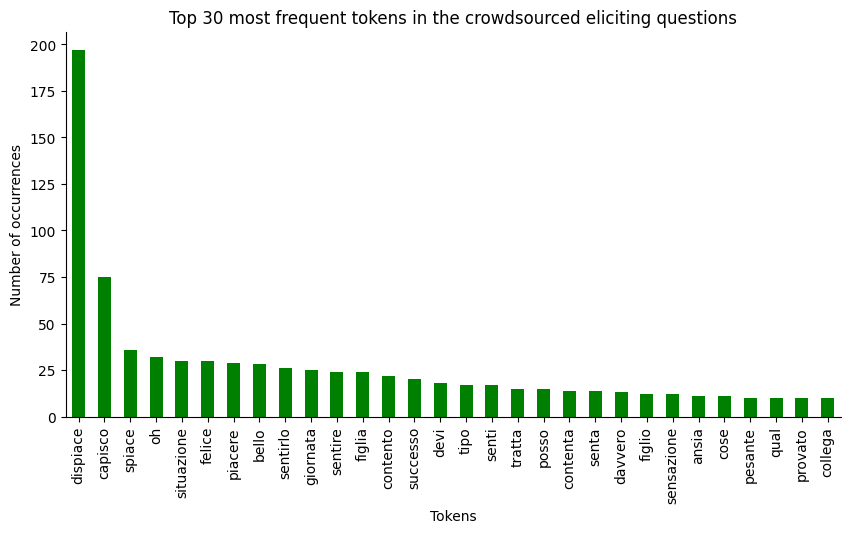
\includegraphics[width=1\linewidth]{assets//imgs/dataset-top-30-answers.png}
    \caption{Bar chart showing the top 30 most frequent tokens present in the crowdsourced eliciting questions. Notice how tokens such as \emph{``dispiace"} are very common. This aligns with our guidelines of showing empathy for sad narratives. }
    \label{fig:dataset-top-30-answers}
\end{figure}

In Figure \ref{fig:dataset-top-30-answers}, a bar chart representing the top 30 most frequent tokens from the collected eliciting questions are shown. The most prevalent token is \emph{``dispiace"}, which occurs disproportionately frequently with respect to the other tokens. This observation aligns coherently with the guidelines, which emphasise the importance of conveying empathy, especially for narratives of a sorrowful nature, which constitute the majority of the dataset.

Additionally, an analysis of the time employed by the crowdworkers to complete the task and the length of their assigned narratives was done. Initially, our hypothesis posited a strong correlation between the length of a narrative and the corresponding time required for writing an eliciting question to continue the narrative. We anticipated that users would invest more time comprehending the provided information, resulting in increased time spent on each narrative continuation eliciting question.
\begin{figure}[!htbp]
    \centering
    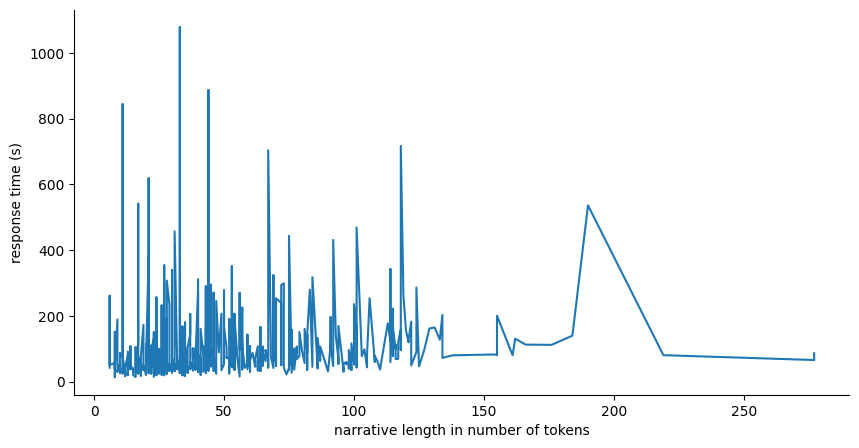
\includegraphics[width=1\linewidth]{assets//imgs/dataset-pearson-correlation.png}
    \caption{Image showing the plot of the correlation between lengths of the narratives (x-axis) and the corresponding time required to elicit (y-axis). For most narratives, the narrative length does not influence the completion time, as the bulk of the response times are under 200s regarless of narrative length. Response time is the time from when the narrative is shown to the user to them sending the answer. }
    \label{fig:dataset-pearson-correlation}
\end{figure}
% \begin{figure}[!htbp]
%     \centering
%         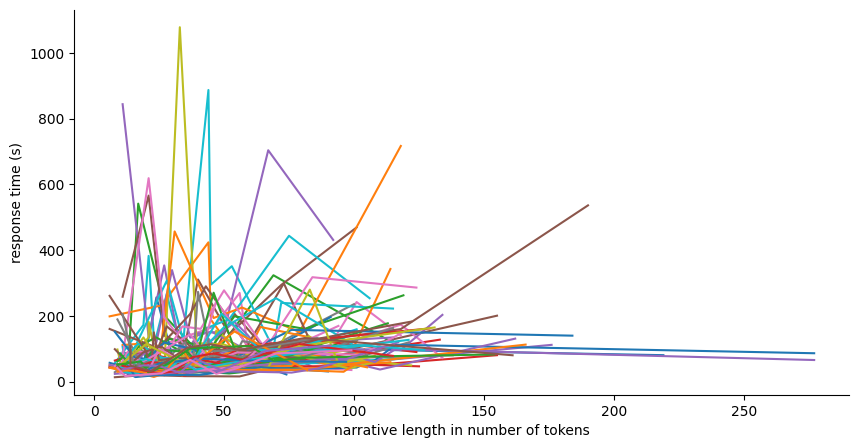
\includegraphics[width=1\linewidth]{assets//imgs/dataset-overall-correlation-workers.png}
%         \caption{In Figure is shown the correlation between lengths of the narratives (x-axis) and the corresponding time required to elicit (y-axis). It is possible to notice that most annotators are able to complete each task within 200 seconds, regardless of the narrative length.}
%         \label{fig:dataset-overall-correlation-workers}
% \end{figure}
However, it was found that this is not to be the case, as pictured in Figure \ref{fig:dataset-pearson-correlation}. To provide a more precise quantification of this observation, the Pearson correlation coefficient \cite{pearson} was computed between the completion times for each narrative and the respective narrative lengths. The resulting overall correlation coefficient was found to be 0.16, further supporting the notion that completion times and narrative lengths do not exhibit a linear relationship. This is likely the result of the human annotators spending time carefully considering their proposed questions after reading the narrative rather than simply reading the narrative and immediately responding. This is further supported by the fact that the majority of the crowdworkers completed the task within 200 seconds, regardless of the narrative length.

\begin{figure}[!htbp]
        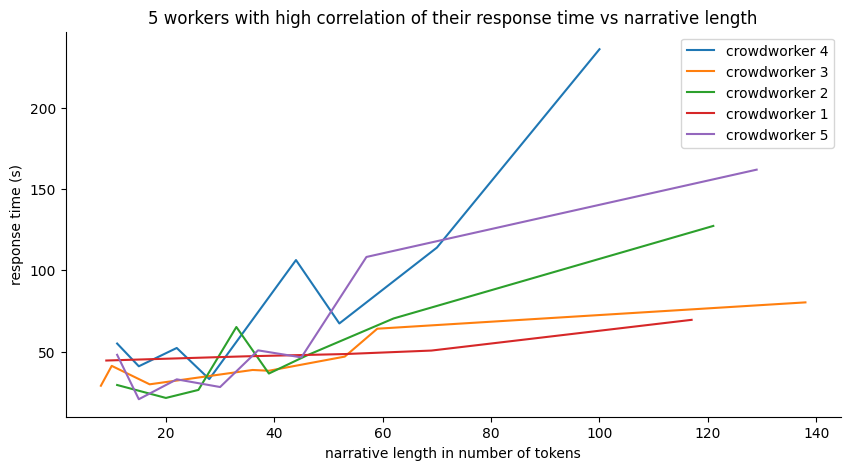
\includegraphics[width=1\linewidth]{assets//imgs/dataset-high-correlation-workers.png}
        \caption{Image reporting the correlation between lengths of the narratives (x-axis) and the corresponding time required to elicit (y-axis) for 5 workers in particular. For these 5 annotators, there is a high degree of linear correlation between the narrative length and the time required for completion.}
        \label{fig:dataset-high-correlation-workers}
\end{figure}
Nevertheless, although this result is true on the whole dataset and for most crowdworkers, it is important to note that a few outliers were encountered. These crowdworkers exhibited a notably strong correlation. As illustrated in Figure \ref{fig:dataset-high-correlation-workers}, these specific users displayed a correlation coefficient exceeding 0.90. We attribute this phenomenon to the exceptional speed with which these users crafted their responses, which in turn placed a significant emphasis on the reading time as the dominant factor in their overall response time.

\begin{table}[!htbp]
\centering
\caption{Examples of eliciting questions for two narratives are reported on each row. Narratives are reported in the first column and corresponding eliciting questions are reported in the second column. On the top a longer narrative with two different eliciting questions. Notice that eliciting questions for the longer narrative pursue different topics. On the bottom is a shorter narrative, with more eliciting questions but on the same few set of topics.}
\label{tab:personal-narrative-elicitation-continuations-example}
    \centering
    \begin{tabularx}{\linewidth}{ l|X | X  }
    % \begin{tabular}{p{1.5cm}|p{3cm}|p{5cm}|p{2.5cm}|p{2cm}}
        \toprule
        \multicolumn{3}{c}{\thead{Examples of narrative and respective eliciting questions}} \\
        \midrule
        % \thead{Mode}
        % \midrule
        \thead{Example}& \thead{Narrative} & \thead{Crowdsourced Eliciting Questions} \\
        \midrule
        \thead{1} & \multirow{2}{7cm}{Giornata piacevole ma stancante. Comunione di una nipotina. Oggi non è stata una giornata abbastanza calda ... mangiare al freddo non è il massimo. Non ero emozionata sapendo dove era il posto ... mi sono coperta per quanto possibile visto il periodo.} &  Congratulazioni per il bellissimo evento. La tua nipotina è stata felice? \\
 [2em]
       %        \cmidrule{2-2}
        && Se non altro hai allenato il tuo spirito di adattamento. Spero che la giornata sia andata bene, eri contenta alla fine della giornata? \\
        \arrayrulecolor{black}
        \midrule
        \thead{2 } & \multirow[t]{10}{*}{Che noia finiranno le feste?} & Mi spiace tu ti annoi, come mai?\\
 [1em]
       %        \cmidrule{2-2}
        && Ti capisco. Come mai non ti piacciono?\\
 [1em]
       %        \cmidrule{2-2}
        && Capisco, immagino che hai trascorso delle belle giornate!\\
 [2em]
       %        \cmidrule{2-2}
        && Mi dispiace non ti piacciano, perché vuoi che finiscano?\\
 [2em]
       %        \cmidrule{2-2}
        && Mi dispiace, che cosa hai fatto durante le feste che ti ha annoiato?\\
 [2em]
       %        \cmidrule{2-2}
        && Mi spiace tu stia così, che cosa ti causa noia in queste feste?\\
 [2em]
       %        \cmidrule{2-2}
        && Mi dispiace che ti annoi, perché vuoi che finiscano?\\     
 [1em]
       %        \cmidrule{2-2}
        && Concordo, quando ricominci a lavorare tu?\\      
 [1em]
       %        \cmidrule{2-2}
        && Ti capisco, per quale motivo ti senti annoiato?\\      
 [1em]
       %        \cmidrule{2-2}
        && Mi dispiace che le feste ti annoino, come mai non ti piacciono?\\
       \arrayrulecolor{black}
        \bottomrule

    \end{tabularx}
\end{table}
              % "input": "Giornata piacevole ma stancante. Comunione di una nipotina. Oggi non \u00e8 stata una giornata abbastanza calda ... mangiare al freddo non \u00e8 il massimo. Non ero emozionata sapendo dove era il posto ... mi sono coperta per quanto possibile visto il periodo. ",
              %   "output": [
              %       {
              %           "generated_text": "Congratulazioni per il bellissimo evento. La tua nipotina \u00e8 stata felice? "
              %       },
              %       {
              %           "generated_text": "Se non altro hai allenato il tuo spirito di adattamento. Spero che la giornata sia andata bene, eri contenta alla fine della giornata?"
              %       }
              %   ],
              %   "id": "264"
              %               {
              %   "input": "Che noia finiranno le feste? ",
              %   "output": [
              %       {
              %           "generated_text": "Mi spiace tu ti annoi, come mai?"
              %       },
              %       {
              %           "generated_text": "Ti capisco. Come mai non ti piacciono?"
              %       },
              %       {
              %           "generated_text": "Capisco, immagino che hai trascorso delle belle giornate!"
              %       },
              %       {
              %           "generated_text": "Mi dispiace non ti piacciano, perch\u00e9 vuoi che finiscano?"
              %       },
              %       {
              %           "generated_text": "Mi dispiace, che cosa hai fatto durante le feste che ti ha annoiato?"
              %       },
              %       {
              %           "generated_text": "Mi spiace tu stia cos\u00ec, che cosa ti causa noia in queste feste?"
              %       },
              %       {
              %           "generated_text": "Mi dispiace che ti annoi, perch\u00e9 vuoi che finiscano?"
              %       },
              %       {
              %           "generated_text": "Concordo, quando ricominci a lavorare tu?"
              %       },
              %       {
              %           "generated_text": "Ti capisco, per quale motivo ti senti annoiato?"
              %       },
              %       {
              %           "generated_text": "Mi dispiace che le feste ti annoino, come mai non ti piacciono?"
              %       }
              %   ],
A brief reading of the eliciting questions for a few examples of narratives revealed that most of the annotators propose the same inquiries or topics for short narratives. An example is shown in Table \ref{tab:personal-narrative-elicitation-continuations-example}. We believe this fact is the result of a narrative not having more than one or a few natural directions.% This fact will play an important role in the evaluation of LLMs later in chapter 4.
